\documentclass{chi2009}
\usepackage{times}
\usepackage{url}
\usepackage{graphics}
\usepackage{color}
\usepackage[T1]{fontenc}
\usepackage[pdftex]{hyperref}
\hypersetup{%
pdftitle={Your Title},
pdfauthor={Your Authors},
pdfkeywords={your keywords},
bookmarksnumbered,
pdfstartview={FitH},
colorlinks,
citecolor=black,
filecolor=black,
linkcolor=black,
urlcolor=black,
breaklinks=true,
}
\newcommand{\comment}[1]{}
\newcommand{\img}[2][0.2in]{\includegraphics[height=#1]{figures/#2}}
\newcommand{\cmd}[1]{\textcolor[rgb]{.25,.5,.5}{\textbf{#1}}}
\newcommand{\find}[1]{{\tt find({#1})}}
\newcommand{\findAll}[0]{{\tt findAll()}}
\newcommand{\Pattern}[0]{{\tt Pattern}}
\newcommand{\Region}[0]{{\tt Region}}
\newcommand{\Match}[0]{{\tt Match}}
\newcommand{\click}[0]{{\tt click}}
\newcommand{\type}[0]{{\tt type}}
\newcommand{\dragDrop}[0]{{\tt dragDrop}}

\pagenumbering{arabic}  % Arabic page numbers for submission.  Remove this line to eliminate page numbers for the camera ready copy

\begin{document}
% to make various LaTeX processors do the right thing with page size
\special{papersize=8.5in,11in}
\setlength{\paperheight}{11in}
\setlength{\paperwidth}{8.5in}
\setlength{\pdfpageheight}{\paperheight}
\setlength{\pdfpagewidth}{\paperwidth}

\title{Using Graphical Representation of User Interfaces as Visual References}
\author{Tsung-Hsiang Chang\\
\affaddr{MIT CSAIL}\\
\affaddr{Cambridge, MA}\\
\email{vgod@mit.edu}
}
\date{}
\maketitle

\begin{abstract}
\end{abstract}

\section{Introduction}
In human-to-human communication, asking for information about tangible objects
can be naturally accomplished by making direct visual references to them. For
example, to ask a tour guide to explain more about a painting, we would say
``tell me more about this'' while pointing to \img{paint.png}. 
Giving verbal commands involving
tangible objects can also be naturally accomplished by making similar visual
references. For example, to instruct a mover to put a lamp on top of a
nightstand, we would say “put this over there” while pointing to 
\img{lamp.png}  and \img{cabinet.png} respectively.

However, in human-to-computer communication, most interfaces do not
interact with us visually and force us to rely on non-visual alternatives. One
example is searching for help.  With the explosion of information on the web,
search engines are increasingly useful as a {\it first} resort for help with an
application, because the web may have fresher, more accurate, more abundant
information than the application’s built-in help.  Searching the web currently
requires coming up with the right keywords to describe the GUI element, which
can be challenging.

Another example is GUI automation and testing. 
Scripts or macros that control GUI elements or verify if a GUI
has correct behavior
either refer to an element by name, which may be unfamiliar or even unavailable
to the user, or by screen location, which may change. 
Broadly speaking, non-visual references exist from a 
single GUI element to an application, even to a device.
These non-visual
alternatives present certain limitations to GUI users as they perform 
various kinds of tasks.

In this thesis, we contriubte a series of work that use the graphical
representation of user interfaces (i.e. their screenshots) as
visual references.
Our work introduces new interaction models for
human-to-computer communication
to find information or issue commands involving GUI elements 
by naturally making direct visual reference to them.
We have developed the following systems that embodies this new interaction
concept:

\begin{itemize}
\item Sikuli Search, a system that enables users to search a large collection
of online documentation about GUI elements using screenshots. 
For example, we can search documentations about this tool \img{lasso.png}
in Photoshop by taking a screenshot of it without knowing its name.
\item Sikuli Script, a scripting system that enables programmers to use
screenshots of GUI elements to control them programmatically. The system
incorporates a full-featured scripting language (Python) and an editor
interface specifically designed for writing screenshot-based automation
scripts. With Sikuli Script, we can ask the computer to ``move all Word
documents to the recycle bin'' by using a command \dragDrop{} and taking
screenshots of \img{word.png} and \img{recycle.png} respectively.
\item Sikuli Test, a system based on Sikuli Script that enables Quality 
Assurance (QA) testers to create test scripts to verify GUI behavior without
writing code. 
\item Deep Shot, a framework for capturing the user’s work state that is needed
for a task (e.g., the specific part of a webpage being viewed) and resuming it
on a different device. We introduced two new interaction techniques {\it deep
shooting} and {\it deep posting} with Deep Shot, for pulling and pushing work
states, respectively, using a mobile phone camera. For example,
we can use a mobile phone camera
to take a picture of a desktop monitor showing a map \img{map.png}
and ask the computer to open the same region of the map on the phone.
\end{itemize}

Compared to the non-visual alternatives, taking screenshots is an intuitive way
to specify a variety of GUI elements, applications, or devices. Also,
screenshots are universally
accessible for all applications on all GUI platforms, since it is always
possible to take a screenshot of the interface the users see.
However, graphical representation has its limitations. 
First, 
it may not consist of the complete information we need. For example,
long file names could be abbreviated with "...", but we usually need
the full file names. Second, extracting text from screenshots is hard.
The current OCR technology we used in our works was designed for scanned
papers, which are usually high-resolution black text on white backround
and have simple layouts, but not for text on screens,
which are usually small and have complicated layouts and colored backgrounds.

Therefore, we propose to investigate further in these problems with the 
following projects.
\begin{itemize}
\item Developing a hybrid framework that utilizes both screenshots and 
Accessibility API of modern operating systems. We will also study how
to integrate different sources of GUI information depending on
the scenarios for fast and reliabile searching and text extraction.

\item Improving OCR for screen text. New OCR algorithms need to be developed 
for window-based layout analysis, text detection on backgrounds with different
colors, and text recognition for small text.
\end{itemize}

\section{Thesis Statement}
Graphical representation of user interfaces can be used as direct
visual references to enable new kinds of interaction model in domains
like searching, GUI automation and testing, and cross-device information 
migration.

%Current approaches to user interface automation tend to require support 
%from application developers (e.g.,
%AppleScript and Windows Scripting, which require applications to provide
%APIs) or accessible text labels for GUI elements (e.g. DocWizards \cite{},
%Chickenfoot \cite{}, and CoScripter \cite{}). 
%Some macro recorders (e.g. Jitbit  and
%QuicKeys ) achieve cross-application and cross-platform operability by
%capturing and replaying low-level mouse and keyboard events on a GUI element
%based on its absolute position on the desktop or relative position to the
%corner of its containing window. However, such position may become invalid if
%the window is moved or if the elements in the window are rearranged due to
%resizing.  Therefore, we propose to use screenshots of GUI elements directly in
%an automation script to programmatically control the elements with low-level
%keyboard and mouse input. Since screenshots are universally accessible across
%different applications and platforms, this approach is not limited to a
%specific application. Furthermore, the GUI element a programmer wishes to
%control can be dynamically located on the screen by its visual appearance,
%which eliminates the movement problem suffered by existing approaches.


\subsection{GUI Automation with screenshots}
We have developed Sikuli Script, a visual scripting API for GUI automation. 
The goal of this API is to give an existing
full-featured scripting language a set of image-based interactive capabilities.
While in this thesis we describe the API in Python syntax, adapting it to other
scripting languages such as Ruby and JavaScript should be straightforward.  

The
Sikuli Script API has several components.  The \find{} function 
takes a target
pattern and returns screen regions matching the pattern.  The \Pattern{} and
\Region{} classes represent the target pattern and matching screen regions,
respectively.  A set of action commands invoke mouse and keyboard actions on
screen regions. Finally, a visual hash table stores key-values pairs using
images as keys. We describe these components in more detail below.

\subsubsection{Find}
The \find{} function locates a particular GUI element to interact with. 
It takes
a visual pattern that specifies the element’s appearance, searches the whole
screen or part of the screen, and returns regions matching this pattern or
null if no such region can be found. For example, 
\find{
\includegraphics[height=0.2in]{figures/word.png}}
finds regions containing a Word document icon on the whole screen.)
In addition to \find{}, another function \findAll{} returns all matching
regions instead of the best one.

\subsubsection{Pattern}
The \Pattern{} class is an abstraction for visual patterns. A pattern object can
be created in three ways: from an image file, or
from a string of text. When created from an image, 
we use a computer vision algorithm {\it template matching}
to find matching screen regions.
When created from a string, OCR is used to find screen regions matching the
text of the string.  A pattern object has four methods for tuning how general
or specific matches must be:

\begin{itemize}
\item {\bf exact}(): Regions must match the given pattern exactly.
\item {\bf similar}({\it similarity}): Allow matches that are somewhat different from the
given pattern in visual features. A similarity threshold between 0 and 1
specifies how similar the matching regions must be.
\item {\bf anyColor}(): Allow matches with different colors than the given pattern.
\item {\bf anySize}():  Allow matches of a different size than the given pattern.
\end{itemize}

Each method produces a new pattern, so they can be chained together.  
For example, \\
{\small
\verb|Pattern(|
\includegraphics[height=0.2in]{figures/word.png}
\verb|).similar(0.8).anyColor().anySize()|}.

\subsubsection{Region and Match}
The \Region class defines a rectangular region on a screen.
Its attributes are x and y coordinates, height, width.
The \Match class extends the \Region class and
provides an abstraction for the screen region(s)
returned by the \find function matching a given visual pattern. 
It has an addtional attribute: similarity score.
Typically, a \Match object represents the top match, for example, 
{\tt m = }\find{
\includegraphics[height=0.2in]{figures/word.png}}
stores the region found to look most like the icon in the variable m. 
Another use of a Region object is to
constrain the search to a particular region instead of the entire screen. For
example, 
\find{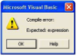
\includegraphics[height=0.4in]{figures/dialog.png}}.\find{
\includegraphics[height=0.15in]{figures/ok.png}}
 constrains the search space of the second find for the
ok button to only the region occupied by the dialog box returned by the first
\find{}. 
To support other types of constrained search, our visual scripting API
provides a versatile set of constraint operators: left, right, above, below,
nearby, inside, outside in 2D screen space and after, before in reading order
(e.g., top-down, left-right for Western reading order). These operators can be
used in combination to express a rich set of search semantics, for example,\\
{\small
\find{
\includegraphics[height=0.2in]{figures/toolbar.png}}{\tt.inside().}\find{
\includegraphics[height=0.2in]{figures/btn1.png}}{\tt.right().}\find{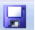
\includegraphics[height=0.2in]{figures/btn2.png}}
}

\subsubsection{Action}
The action commands specify what keyboard and/or mouse events to be issued to
the center of a region found by find(). The core set of commands in our API are:

\begin{itemize}
\item {\bf click}({\it Pattern|Region}), {\bf doubleClick}({\it Region}): 
These two commands issue mouse-click
events to the center of a target region. For example, 
\click(\img{close.png}) performs a
single click on the first close button found on the screen. 
Modifier keys such
as Ctrl and Command can be passed as a second optional argument.

\item {\bf dragDrop}({\it Pattern|Region} target, {\it Pattern|Region} destination): 
This command drags the
element in the center of a target region and drops it in the center of a
destination region. For example, \dragDrop(\img{word.png} ,\img{recycle.png} ) 
drags a word icon and drops it in the recycle bin.

\item {\bf type}({\it Pattern|Region} target, String text): 
This command enters a  given text in a
target region by sending keystrokes to its center. For example, 
\type(\img{google.png} ,"Sikuli")
types the ``Sikuli'' in the Google search box.
\end{itemize}

\subsubsection{Visual Hash Table}
A visual Hash table can be used to store key-value pairs using images as keys.
It uses the same syntax as a
typical Hash table in Python to create tables and to store values that need to
be quickly retrieved (i.e., sub-linear time) by images. 
For example, {\tt h = }\{ \img{word.png} :
"word",  \img{ppt.png} : "powerpoint"\} creates a visual hash table 
associating two
application names with their icon images. 
Then, {\tt h[\img{word.png}]} retrieves the string word,
{\tt h[\img{excel.png}]} = "excel" adds the string "excel" under 
its icon image, and {\tt h[\img{recycle.png}]} returns a null object.


\subsubsection{Sikuli Script Editor}
%TODO: put a new screen shot of Sikuli IDE here
We have developed an editor to help users write visual scripts. The
patterns embedded in each statement are shown as inline images. The editor also
provides code completion. When a programmer types a command, the editor
automatically displays the corresponding command template to remind the
programmer what arguments to supply. For example, when the programmer types
find, the editor will expand the command into \img[0.15in]{find-cam.png}. 
The programmer can click on the
camera button to capture a portion of the screen as a visual pattern. When
taking a screenshot, the editor hides itself automatically to reveal the
desktop underneath. Alternatively, the programmer can load an existing image
file using the toolbar, or type the filename or URL of an image, and the editor
automatically loads it and displays it as a thumbnail.  The editor can also
preview how a pattern matches the current desktop (FIGURE)
%TODO: put preview window here
 under different
parameters such as similarity threshold, so that these can be tuned to include
only the desired regions. Match scores are mapped to the hue and the alpha
value of the highlight, so that regions with higher score are redder and more
visible. The editor also allows programmers to specify an arbitrary region of
screen to confine the search to that region.


\subsection{GUI Testing with screenshots}
Based on Sikuli Script, 
we have developed Sikuli Test, a testing framework that enable 
developers and QA testers to automate GUI testing tasks.
Consider the following task description for testing a particular
GUI feature:

\begin{quote}
Click on the color palette button. Check if the colors dialog
window appears
\end{quote}

To carry out this test case, QA testers need to manually interact
with the GUI and visually check if the outcome is correct. Using
Sikuli Test, the testers can automate this process by converting
the task description into an automation script. This script
consists of action statements to simulate the interactions
and assertion statements to visually verify the outcomes
of these interactions. For example,
the above task description can be easily translated into a test
script as:


\verb|click(|
\includegraphics[height=0.2in]{figures/palette.png}\verb|)|; $\;$
\verb|assertExist(|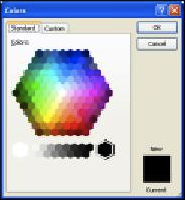
\includegraphics[height=0.4in]{figures/color-dialog.png}\verb|)|;


\begin{figure*}
\center
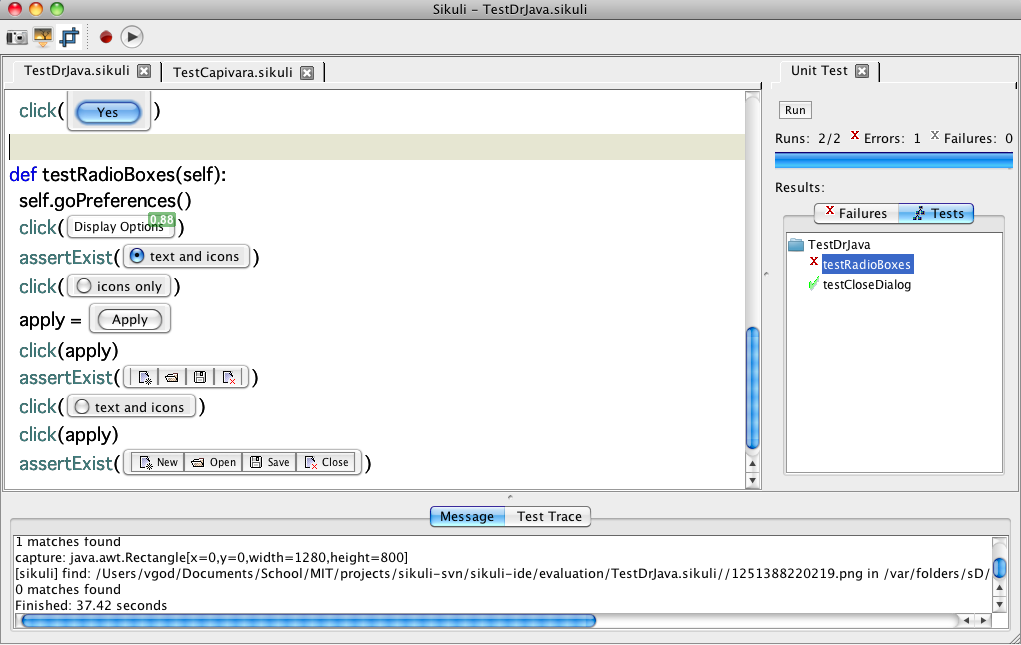
\includegraphics[width=1.5\columnwidth]{figures/editor.png}
\caption{Editor for writing Sikuli Test scripts.}
\end{figure*}

By taking this image-based scripting approach, Sikuli Test 
lowers the barrier to write scripts by
allowsing testers to refer to GUI objects by their
direct visual representation, and to provide robustness to
changes in spatial arrangements of GUI components.

\subsection{Simulating Interactions using Action Statements}

To simulate interactions involved in a test case, QA testers can
write action statements using the syntax defined in Sikuli Script.
Since Sikuli Script is based on a full scripting language,
Python, it is possible for QA testers to programmatically
simulate a large variety of user interactions, no matter simple or
complex.

\subsection{Verifying Outcomes using Assertion Statements}

Sikuli Test introduces two \emph{visual} assertion functions. QA
testers can include these functions in a test script to verify
whether certain GUI interaction generates the
desired visual feedback. These two assertion functions are defined
in the class \verb|Region|:


\verb|assertExist(image or string)| \\
asserts that an
image or string that should appear on screen or in a specific screen region

\verb|assertNotExist(image or string)| \\
asserts that an
image or a string should not appear on screen or in a specific screen region

The \verb|image| is specified as an URL or a path to an image
file. It also can be captured by a screenshot tool provided in our IDE.
When a string is specified, OCR is performed to check if the
specified string can be found in the specific region. 

\subsubsection{Test By Demonstration}
Sikuli Test provides a record-playback utility that enables QA testers to
automate GUI testing by demonstration. The operation of a GUI can be described
as a cycle consisting of actions and feedback. Given a test case, the testers
follow the given actions to operate a GUI, and verify if the visual feedback is
the same as expected. If so, they proceed to do the next actions and to verify
further feedback.  


With the record-playback mechanism, the testers can demonstrate the
interactions involved in the test case. The actions as well as the
screen are recorded and translated into a sequence of action and assertion
statements automatically. The action statements, when being executed, can
replicate the actions, as if the testers are operating the GUI themselves.
Besides, the assertion statements can verify if the automated interactions
lead to the desired visual feedback, as if the testers are looking at the
screen themselves.  The test-by-demonstration capability of Sikuli Test 
minimizes the barrier and effort needed to write test scripts. 



\subsection{Identifying Applications and Devices with screenshots}

\subsection{Universal Automation Framework} 

\section{Evaluation}

\section{Related Work}
{\bf Image-based interaction:}
The idea of supporting interac-tions by analyzing the visual patterns 
rendered on the screen was examined in the late 90’s.  
Potter \cite{Potter99} was the
first to explore this idea and referred to it as direct pixel access and
championed its potential for supporting application-independent end-user
programming. His Triggers system supported novel visual tasks such as
graphical search-and-replace and simulated floating menus. While Triggers can
be configured through an interactive dialog to perform some basic tasks similar
to the Sikuli Script examples presented earlier, it is not a
%TODO give sikuli script examples
full scripting language and does not support fuzzy matching. 
Zettlemoyer \& St. Amant \cite{zettlemoyer99}
described VisMap and VisScript. The former inferred high-level,
structured representations of interface objects from their appearances and
generated mouse and keyboard gestures to manipulate these objects. The later
provided a basic set of scripting commands (mouse-move, single-click,
double-click and move-mouse-to-text) based on the output of VisMap, but was not
integrated with a full-feature scripting language. 
Furthermore, St. Amant et al
\cite{amant00} explored several possibilities of programming-by-example 
through visual generalization by observing user behaviors and inferring general
patterns based on the visual properties and relationships of user interface
objects. While
these early pioneering works shed light on the potential of image-based
interaction, they led to almost no follow-up work, mostly because the
practicality was limited by the hardware and computer vision algorithms of the
time. However, faster hardware and recent advances in vision algorithms
particularly those based on invariant local features have now presented us with
an opportunity to reexamine this idea and develop practical image-based
interactive applications.

{\bf GUI testing:}


\section{Schedule}
\section{Conclusions}

\bibliographystyle{abbrv}
\bibliography{google-proposal}


\end{document}
